\section{MIMO identification}
Next we are interested in estimating the complete bicycle equations. The system has two inputs; rolling torque $T_\phi$ and steering torque $T_\delta$. The following outputs are measured; roll angle $\phi$ and steerangle $\delta$. Since the system has multiple inputs and multiple outputs we have to apply MIMO system identification techniques. The corresponding block diagram is shown below:
	\begin{center}
		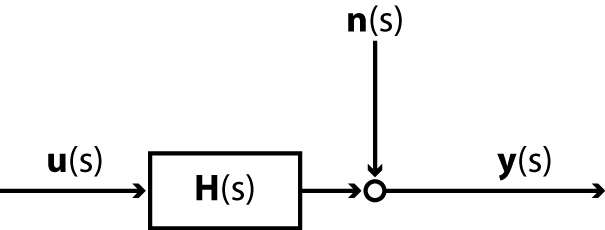
\includegraphics{images/MIMOblock}
		%		\caption{Blockdiagram of the SISO model}
		\label{fig:MIMOblock}
	\end{center}
Where $\mathbf{u} = \mathbf{u}(s)$ represents the input vector, $\mathbf{y}= \mathbf{y}(s)$ represents the measured output vector and $\mathbf{n} = \mathbf{n}(s)$ represents the measurement noise vector. The block diagram looks pretty similar to the SISO case, except here the scalar function are replaced by vectors and matrices.
\subsection{Simulation}
Again the linearized benchmark equations are used for the simulation. A forward velocity of 5 m/s is chosen, which results in stable dynamic behavior of the bicycle. The governing input/output relationship is shown below in state space form:
	\begin{align}
		\mathbf{\dot{x}} & = \mathbf{A}\mathbf{x} + \mathbf{B}\mathbf{u} \nonumber \\
		\mathbf{y} & = \mathbf{C}\mathbf{x} 
	\end{align}
Where;
	\begin{align}
	{\scriptstyle
			\mathbf{A} =   \left[\begin{array}{cccc} 
									$0$ & $0$ & $1$ & $0$ \\
									$0$ & $0$ & $0$ & $1$ \\
									$9.470$ & $-22.758$ & $-0.520$ & $-1.638$ \\
									$12.400$ & $-19.499$ & $18.089$ & $-15.694$   
			\end{array}\right]   \nonumber \ \ , \
			\mathbf{B} = \left[\begin{array}{cc}
									 $0$ & $0$ \\
									$0$ & $0$ \\
									$0.016$ & $-0.123$ \\
									$-0.123$ & $4.265$ 
			\end{array}\right] \nonumber \ \ , \ 
			\mathbf{C} = \left[\begin{array}{cccc}
									$1$ & $0$ & $0$ & $0$ \\
									$0$ & $1$ & $0$ & $0$
			\end{array}\right]  \nonumber
	}
	\end{align}
A simulation is set up, using the same measurement parameters as for the SISO case (see table: \ref{table:SISOparms}. The input signal $\mathbf{u}$ is designed as an crested multisine which will be explained later on in more detail. The maximum steering torque is set to 0.6 Nm and the maximum roll torque is set to 10 Nm. The standard deviation of the noise for all measured outputs is set to 0.01 rad. The simulation is run twice, with different input vectors. 
\subsection{MIMO system identification}
Next we will use the simulated dataset to derive the transfer function of the system. Starting from the block diagram shown in figure \ref{fig:MIMOblock} we can derive the following equation:
\begin{align}
		\mathbf{H}\mathbf{u} & = \mathbf{y}-\mathbf{n} 
\end{align}
Unfortuneatly this system is not solvable, since we can't invert the inputvector $\mathbf{u}$. Therefore we need additional measurements. A nice choice of input would be the following:
\begin{align}
		\mathbf{U}(s) = \left[\begin{array}{cc}
									A_\phi &  A_\phi \\
									A_\delta & -A_\delta \\
			\end{array}\right] u(s)
\end{align}
Where $A_\phi=5$ and $A_\delta=0.6$ are amplification gains which are found by trial and error. Similar as in the SISO case we will seek a solution in the image of $\mathbf{U}$. Here only need to be a little bit more carefull, since the multiplication of vectors and matrices is generally non-communicative.
\begin{align}
		\mathbf{H}\mathbf{U} & = \mathbf{Y}-\mathbf{N}  \nonumber \\
		\mathbf{U}^\ast\mathbf{H}^\ast & = \mathbf{Y}^\ast-\mathbf{N} ^\ast \nonumber \\
			\mathbf{U}\mathbf{U}^\ast\mathbf{H}^\ast & = 	\mathbf{U}\left(\mathbf{Y}^*-\mathbf{N} ^\ast\right) \nonumber \\
			\mathbf{H}^\ast & = 	\left(\mathbf{U}\mathbf{U}^\ast\right)^{-1}\mathbf{U}\left(\mathbf{Y}^\ast-\mathbf{N} ^\ast\right) \nonumber \\
						\mathbf{H} & = 	\left(\mathbf{Y}-\mathbf{N}\right)\mathbf{U}^\ast\left(\mathbf{U}\mathbf{U}^\ast\right)^{-1} 
\end{align}
Next we define the estimated transferfunction $\hat{\mathbf{H}}$ to be the transferfunction that linearly correlates the input/output data, assuming that the input is independent of the noise ($\mathbf{N}\mathbf{U}^\ast \approx \mathbf{0}$). 
\begin{align}
						\hat{\mathbf{H}} 	= & \mathbf{Y}\mathbf{U}^\ast\left(\mathbf{U}\mathbf{U}^\ast\right)^{-1} \nonumber \\
																			= & \mathbf{S}_{yu}\mathbf{S}_{uu}^{-1}
		\label{eq:MIMOH}
\end{align}
Here $S_{uy}$ represent the cross spectral density of the input/output and $S_{uu}$ represents the auto spectral density of the input. The resulting tranferfunction is shown as a bode function in figure \ref{fig:SISObode}. The gain of the transfer function decreases as the frequency increases, resulting in a poorer signal to noise ratio at higher frequencies. Also notice that the input signal contains frequency content ranging from 0 to 2 Hz. Above 2 Hz the response is dominated completly by the noise. The coherence represents the linear estimation quality of the transfer function. As expected, the coherence drops dramatically above 2 Hz.
	\begin{figure}
		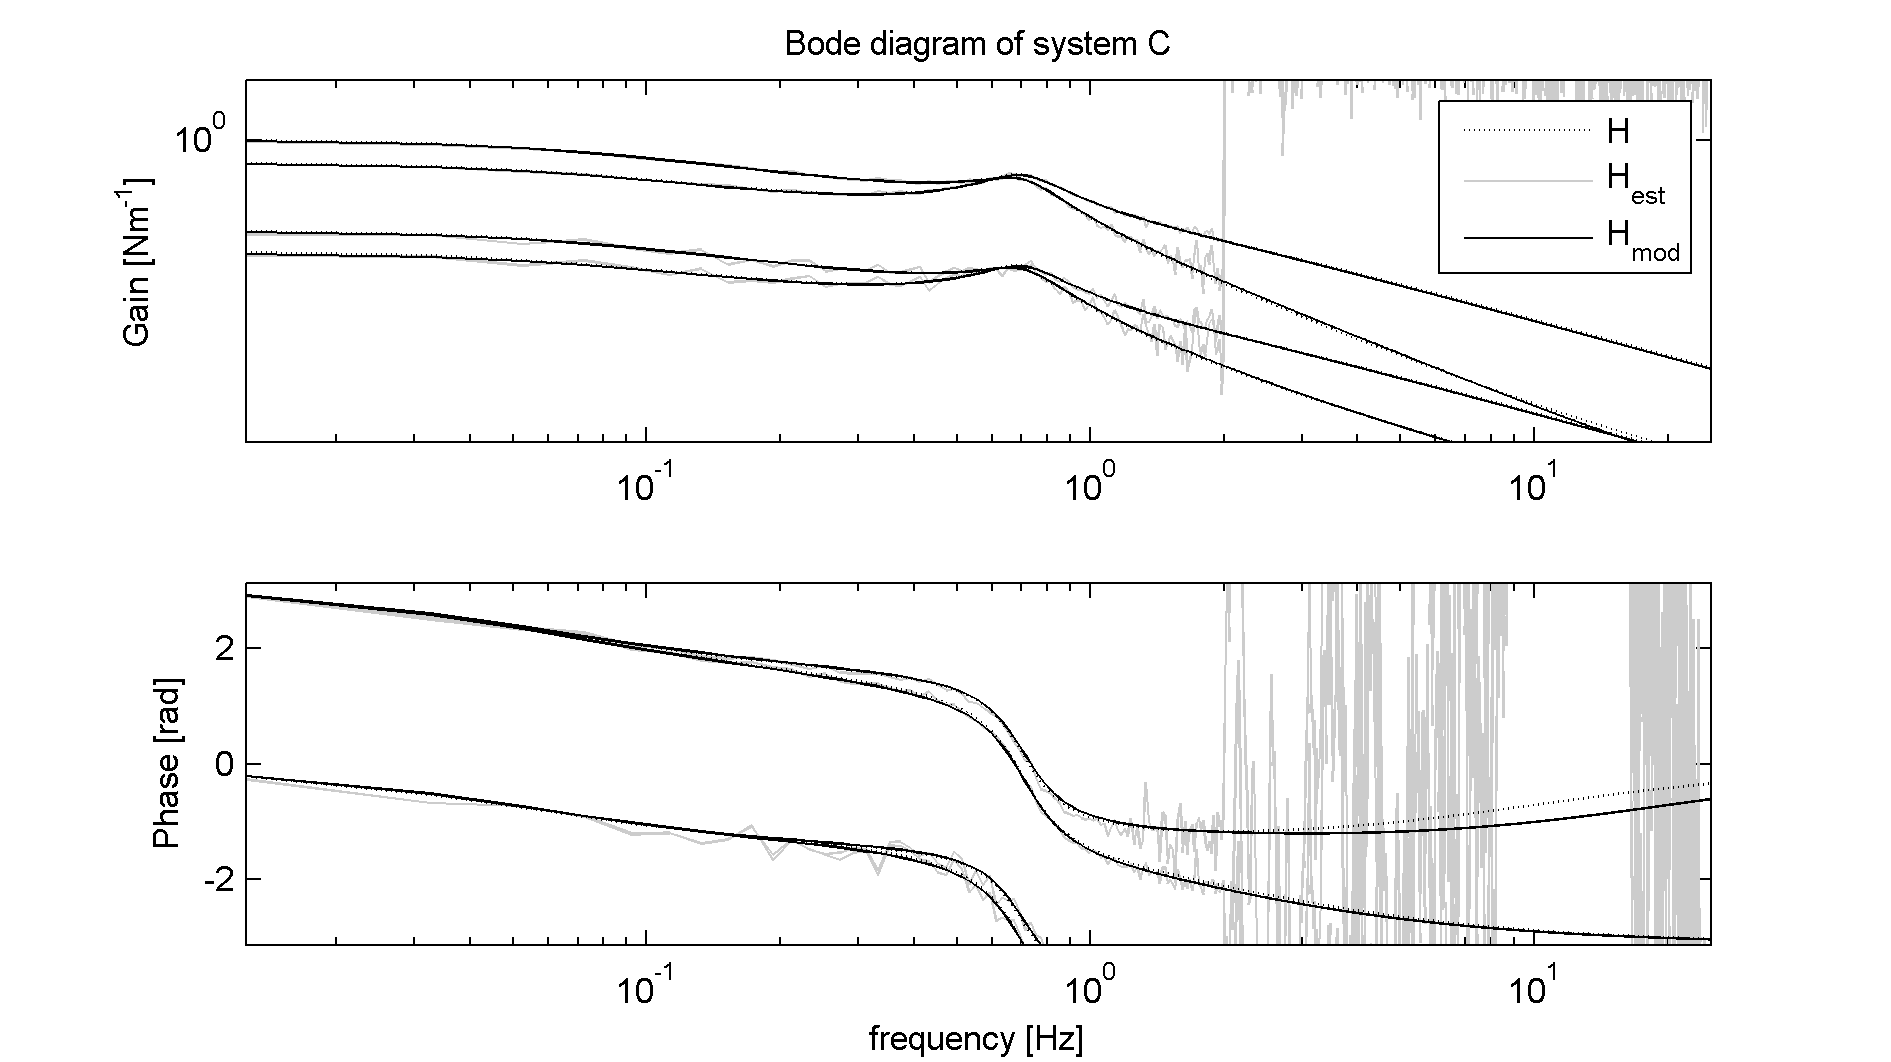
\includegraphics{images/MIMObode}
		\caption{Bode diagram of the true ($H$), estimated ($H_{est}$) and parametric ($H_{mod}$) transfer function.}
				\label{fig:MIMObode}
	\end{figure}
	\subsection{MIMO parameter estimation}
	Yet to be done.